\documentclass[TheoreticalPhy_ModB.tex]{subfiles}
\begin{document}

\chapter{Weak Interactions}

In this section we begin our study of weak interactions. The electroweak theory is described by the Standard Model (SM). However, the full structure of the SM is only revealed at energies comparable to the masses of the bosons $W^\pm$ and $Z^0$ that, together with the photon, mediate the electroweak interactions. Since $m_W=80.425(38)$GeV and $m_Z=91.1876(21)GeV$, the weak decays of particles with masses between a few hundred MeV and a few GeV, as for istance the muons, the pions, the kaouns, the neutron, charmed mesons like the $D^0$, etc., can be studied in a low-energy approximation to the SM. For instance in the $\beta$-decay of the free neutron, $n\to pe^-\var\nu_e$, we have a mass difference $m_n-m_p\simeq1.29$ MeV. Therefore, even if at the funamental level the decay is mediated by the $W$-boson, the fact that the maximum momentum transfer is much smaller than $m_W$ allows un to use a low-energy effective theory. The same approximation holds for nuclear $\beta$- decays. 

For the same reason, we can use the low-energy theory when we study a scattering process mediated by weak interactions, as for instance $e^-\nu_e\to e^-\nu_e$, at center-og-mass energies well below $m_W$.

\skipline

The Weak interactions theory was born after, in the study of $\beta$-deday\footnote{Which theory was developed by Pauli in 1934.}, scientist discovered a process that couldn't be described by QED:
\[n\to p+e^-+\bar \nu_e\]
where $n$ is the neutron, $p$ is the proton, $e^-$ is the electron and $\bar\nu_e$ is the antineutrino. 
From the energy spectrum of out-coming $e^-$ particles scientist understood that this is a 3 body decay. Notice also that netrunos ($\nu_e$ and $\bar \nu_e$) are fermions that couldn't be discovered by detectors since they have no charge. This is the sketch of this interaction:\footnote{We used different colors for different charge currents and different line thickness to distinguish nucleons by smaller fermions.}
\[
\begin{tikzpicture}[baseline=(e0)]
\begin{feynman}[large]
\vertex[blob](e0){\hspace{1cm}};
\vertex[left=of e0](n){$n$};
\vertex[above right=of e0](p){$p$};
\vertex[right=of e0](e){$e^-$};
\vertex[below right=of e0](nu){$\bar\nu_e$};
\diagram*{
	(n) --[fermion, ultra thick](e0),
	(e0) --[fermion, ultra thick, red](p),
	(e0)--[fermion, blue](e),
	(nu)--[fermion](e0),
};
\end{feynman}
\end{tikzpicture}
\]

This new interaction can't be described using QED and two photons that mediate the interactions because of the charge and the spin conservation. 

Beside the neutron decay, much other processes involving weak interaction was found, for example:
\begin{alignat*}{3}
&\text{Leptonic}\hspace{2cm}
&&\mu^-&&\to\, e^-\bar\nu_e\nu_\mu\\
&\text{Semileptonic}
&&n&&\to\, pe^-\bar\nu_e\\
&&&\pi^\mp&&\to\,\mu^\mp\overset{(-)}{\nu}_\mu\\
&\text{Hadronic}
&&\Lambda&&\to\, p\pi^-\\
&&&K^+&&\to\,\pi^+\pi^0
\end{alignat*}

\section{Four Fermions Fermi Lagrangian and neutron decay}
\textsf{Halzen sec 12.1; Maggiore sec. 8.1, 8.2}\\

In 1934 Fermi proposed his theory to describe $\beta$-decay process $n\to p+e^-+\bar \nu_e$. While in QED, the Legrangian for $p\to p\gamma$ (the proton being in a nucleus) is
\[\mathcal L=e(\bar p\gamma^\mu p)A_\mu\]
Fermi replaced the proton current by a current with the transition $n\to p$ and the photon $A_\mu$ by a current expressing the creation of the electron and neutrino:
\[\mathcal L_{\text{W.I.}}=\frac{G_F}{\sqrt 2}\p{\bar p\gamma^\mu n}\p{\bar e \gamma_\mu\nu_e}\]
the constant $e$ being replaced by $G_F$ is called \textbf{Fermi constant}. Here $\bar f$ is the adjoint of the field $f$ for the particle $f$. This lagrangian shows two currents, one related to hadrons $n$ and $p$ called \textbf{hadronic current} and one related to leptons $e$ and $\nu_e$ called \textbf{leptonic current}. It describes 4 fermions interaction. A new coupling constant meant a new force was born. Moreover, the currents in the latter Lagrangian are charged while in QED they are always neutral. Perturbation theory based on this Lagrangian described preatty well the $\beta$-decay.

Since lagrangian has to be 4-dimensional and all these fields have dimension $3/2$ the Fermi constant must have dimension
\[[G_F]=4-6=-2\]
i.e. this theory is not renormalizable since $D=2+2V-E_B-3E_F/2>0$. We will use the SM to obtain a renormalizable theory of weak interactions. 

\subsection{Modifiation of Fermi's theory: the $V$ - $A$ current}
In 1957 Wu found a Parity violation ($\slashed P$) in Weak interaction, since the $e^-$ produced in the neutron decay is mostly left handed. The parity violation signed the death of Fermi's theory. Therefore the Lagrangian must be modified in order to include parity violation. Parity violation is obtained by a mixture of vector current
\[j_V^\mu=\bar e\gamma^\mu \nu_e\]
and an axial current
\[j^\mu_A=\bar e_L\gamma^\mu\nu_e=\bar e\gamma^\mu_L\nu_e=\bar e_L\gamma^\mu\p{\nu_e}_L\]
in particular we have to introduce a current
\[j^\mu=c_Vj^\mu_V-c_Aj^\mu_A=\bar e\gamma^\mu(c_V-c_A\gamma_5)\nu_e\]
Since $e^-$ has both chiralities\footnote{In QED $\bar e\gamma^\mu e=\bar e_R\gamma^\mu e_R+\bar e+L\gamma^\mu e_L$} then I obtain that neutrino has to be only left-handed. Usually I chose $c_V=c_A=1/2$ in order to obtain $(c_V-c_A\gamma_5)=P_L$. Introducing this current in the Fermi Lagrangian I obtain the \text{Four Fermions V-A}\footnote{It is said "V minus A".} interaction for the neutron decay:
\[\mathcal L_{\text{V-A}}^n=-\frac {G_F}{\sqrt2} \p{\bar p\gamma^\mu\p{1-c_A\gamma_5} n}\p{\bar e \gamma_\mu\p{1-\gamma_5}\nu_e}\]
where we modified both hadronic and leptonic currents. Parameter $c_A$ will be fixed by further experiments.

For leptonic processes involving electrons, muons, and them corresponding neutrinos (such as muon decay $\mu^-\to e^-\bar\nu_e\nu_\mu$) we can obtain a similar solution:

\[\mathcal L_{\text{V-A}}^{\mu^-}=-\frac {G_F}{\sqrt2} \p{\bar \nu_\mu\gamma^\alpha (1-\gamma_5)\mu}\p{\bar e \gamma_\alpha (1-\gamma_5)\nu_e}\]

The general form for V-A Lagrangian for leptonic interactions is
\begin{align*}
\mathcal L_{V-A}
&=-\frac{4G_F}{\sqrt2}\p{\sum_{l=e,\mu,\tau}J_L^{\alpha}(l)}^\dagger\p{\sum_{l=e,\mu,\tau}J_{L,\alpha}(l)}
\end{align*}
with
\[J_L^{\alpha}(l)=\bar l\gamma^\alpha P_L\nu_l\]

\subsection{$\mu$-decay and 3-body final state}
\textsf{Maggiore, problem 8.1; Mandl, sec. 16.6.1}\\

Let's consider muon decay rate using V-A lagrangian, $\mu^-\to e^-\bar \nu_e\nu_\mu$. Here there is a sketch of the process, where lines are related to conserved currents in the lagrangian:

\begin{figure}[H]
\centering


\tikzset{every picture/.style={line width=0.75pt}} %set default line width to 0.75pt        

\begin{tikzpicture}[x=0.75pt,y=0.75pt,yscale=-1,xscale=1]
%uncomment if require: \path (0,300); %set diagram left start at 0, and has height of 300

%Curve Lines [id:da8199430993594923] 
\draw    (69.5,151) .. controls (139.5,151) and (177.5,150) .. (188.5,147) .. controls (199.5,144) and (242.5,119) .. (266.5,85) ;
\draw [shift={(129.26,150.63)}, rotate = 539.1700000000001] [fill={rgb, 255:red, 0; green, 0; blue, 0 }  ][line width=0.08]  [draw opacity=0] (8.93,-4.29) -- (0,0) -- (8.93,4.29) -- cycle    ;
\draw [shift={(231.84,120.65)}, rotate = 502.26] [fill={rgb, 255:red, 0; green, 0; blue, 0 }  ][line width=0.08]  [draw opacity=0] (8.93,-4.29) -- (0,0) -- (8.93,4.29) -- cycle    ;
%Curve Lines [id:da968566408247397] 
\draw    (245,243) .. controls (216,194) and (185,158) .. (192,153) .. controls (199,148) and (211,150) .. (340,150) ;
\draw [shift={(216.3,198.24)}, rotate = 236.02] [fill={rgb, 255:red, 0; green, 0; blue, 0 }  ][line width=0.08]  [draw opacity=0] (8.93,-4.29) -- (0,0) -- (8.93,4.29) -- cycle    ;
\draw [shift={(265.79,149.78)}, rotate = 0.32] [fill={rgb, 255:red, 0; green, 0; blue, 0 }  ][line width=0.08]  [draw opacity=0] (8.93,-4.29) -- (0,0) -- (8.93,4.29) -- cycle    ;
%Flowchart: Connector [id:dp043666729593928144] 
\draw  [color={rgb, 255:red, 0; green, 0; blue, 0 }  ,draw opacity=1 ][fill={rgb, 255:red, 0; green, 0; blue, 0 }  ,fill opacity=1 ] (190.5,150.5) .. controls (190.5,150.22) and (190.28,150) .. (190,150) .. controls (189.72,150) and (189.5,150.22) .. (189.5,150.5) .. controls (189.5,150.78) and (189.72,151) .. (190,151) .. controls (190.28,151) and (190.5,150.78) .. (190.5,150.5) -- cycle ;
%Straight Lines [id:da21277212072154672] 
\draw    (112.5,137) -- (141.5,137) ;
\draw [shift={(143.5,137)}, rotate = 180] [color={rgb, 255:red, 0; green, 0; blue, 0 }  ][line width=0.75]    (10.93,-3.29) .. controls (6.95,-1.4) and (3.31,-0.3) .. (0,0) .. controls (3.31,0.3) and (6.95,1.4) .. (10.93,3.29)   ;
%Straight Lines [id:da7169410729564696] 
\draw    (293.5,142) -- (322.5,142) ;
\draw [shift={(324.5,142)}, rotate = 180] [color={rgb, 255:red, 0; green, 0; blue, 0 }  ][line width=0.75]    (10.93,-3.29) .. controls (6.95,-1.4) and (3.31,-0.3) .. (0,0) .. controls (3.31,0.3) and (6.95,1.4) .. (10.93,3.29)   ;
%Straight Lines [id:da2318074943395163] 
\draw    (215,212) -- (231.41,237.32) ;
\draw [shift={(232.5,239)}, rotate = 237.05] [color={rgb, 255:red, 0; green, 0; blue, 0 }  ][line width=0.75]    (10.93,-3.29) .. controls (6.95,-1.4) and (3.31,-0.3) .. (0,0) .. controls (3.31,0.3) and (6.95,1.4) .. (10.93,3.29)   ;
%Straight Lines [id:da9531706570820151] 
\draw    (239,105) -- (262.13,80.46) ;
\draw [shift={(263.5,79)}, rotate = 493.3] [color={rgb, 255:red, 0; green, 0; blue, 0 }  ][line width=0.75]    (10.93,-3.29) .. controls (6.95,-1.4) and (3.31,-0.3) .. (0,0) .. controls (3.31,0.3) and (6.95,1.4) .. (10.93,3.29)   ;

% Text Node
\draw (74,161) node    {$\mu $};
% Text Node
\draw (130,119) node    {$p$};
% Text Node
\draw (244,79) node    {$q$};
% Text Node
\draw (212,232) node    {$p'$};
% Text Node
\draw (313,125) node    {$q'$};
% Text Node
\draw (281,72) node    {$\nu _{\mu }$};
% Text Node
\draw (263,241) node    {$e^{-}$};
% Text Node
\draw (355,145) node    {$\overline{\nu }_{e}$};


\end{tikzpicture}
\end{figure}

Instead of using Feynman diagrams, we prefer to use direct computation from the interaction lagrangian, since Feynman diagrams involve more work due to the product of two different diagrams. Therefore:
\begin{align*}
S_{fi}^{(\mu)}
&=\bra{e(p')\bar\nu_e(q')\nu_\mu(q)}\p{-i\int\de^4x\mathcal L_{\text{V-A}}(x)}\ket{\mu(p)}\\
&=-i\frac{G_F}{\sqrt2}\int\de^4x\bra{e(p')\bar\nu_e(q')\nu_\mu(q)}\p{\bar \nu_\mu\gamma^\alpha_L\mu}_x\p{\bar e \gamma_{\alpha,L}\nu_e}_x\ket{\mu(p)}\\
&=(2\pi)^4\delta^4(p-p'-q'-q)\mathcal M_{fi}
\end{align*}

with

\[\mathcal M_{fi}=-i\frac{4G_F}{\sqrt2}\p{u_{\nu_\mu}(q)\gamma^\alpha_Lu_\mu(p)}\p{\bar u_e(p')\gamma_{\alpha,L}v_{\nu_e}(q')}\]
where we introduced Dirac spinors $u_f$ and $\bar u_f$ for each particle $f$. The unpolarized amplitude reads
\[\overline{|\mathcal M|}^2
=\frac12\p{\frac{4G_F}{\sqrt2}}^2\Tr[(\slashed p+m_\mu)\gamma^\beta_L\slashed q\gamma^\alpha_L]\Tr[(\slashed p'+m_e)\gamma_{\alpha,L}\slashed q'\gamma_{\beta, L}]\]
where we assumed vanishing neutrinos masses since $m_{\nu_e}\simeq m_{\nu_\mu}\approx 10^{-6}m_e$. Using traces proprieties we obtain
\[\overline{|\mathcal M|}^2
=\frac18\p{\frac{4G_F}{\sqrt2}}^2\underbrace{\Tr[\slashed p\gamma^\beta\slashed q\gamma^\alpha(1-\gamma_5)]}_{\tiny\circled A}\underbrace{\Tr[\slashed p'\gamma_{\alpha}\slashed q'\gamma_{\beta}(1-\gamma_5)]}_{\tiny\circled B}\]
which terms can be simplified using Levi-Civita tensor and another tensor:\todo{Is S symmetric?}
\begin{align*}
{\tiny\circled A}&=4\p{S^{\rho\beta\sigma\alpha}-i\epsilon^{\rho\beta\sigma\alpha}}p_\rho q_\sigma\\
{\tiny\circled B}&=4\p{S_{\rho'\alpha\sigma'\beta}-i\epsilon_{\rho'\alpha\sigma'\beta}}(p')^{\rho'}(q')^{\sigma'}
\end{align*}
Contracting tensors we obtain 
\[\overline{|\mathcal M|}^2
=64G_F^2(p\cdot q')(q\cdot p')\]

We can now compute the differential decay rate in the lab frame:
\[\p{\de\overline\Gamma}_{\text{LAB}}
=\frac{\overline{|\mathcal M|}^2_{\text{LAB}}}{2m_\mu}\de\Phi_{(3)}\]
where $\de\phi_{(3)}$ is the three body phase space:
\[\de\Phi_{(3)}=(2\pi)^4\delta^4(p-p'-q'-q)
\p{\frac{\de^3p'}{(2\pi)^32\omega_e'}}
\p{\frac{\de^3q'}{(2\pi)^32\omega_{\nu_e}'}}
\p{\frac{\de^3q}{(2\pi)^32\omega_{\nu_\mu}}}
\]
Notice that since I cannot see neutrino experimentally, I can't measure the energies of neutrinos separately.
If we define
\[k=(p-p')=(q+q')\]
then
\[\p{\de\overline\Gamma}_{\text{LAB}}
=\frac{4G_F^2}{(2\pi)^5}\frac{p_\alpha p'_\beta}{m_\mu}\frac{\de^3p'}{\omega_e'}I^{\alpha\beta}(k)
\]
where we introduced the following tensor
\begin{align*}
I_{\alpha\beta}(k)
&=\int\frac{\de^3q'}{\omega_{\nu_e}'}\frac{\de^3q}{\omega_{\nu_\mu}}\delta^4(p-p'-q'-q)q'_\alpha q_\beta\\
&=g_{\alpha\beta}A(k^2)+\frac{k_\alpha k_\beta}{k^2}B(k^2)
\end{align*}
for some functions $A(k^2)$ and $B(k^2)$. Using tensor proprieties we have
\begin{equation}\label{eqn:mu-decay-tensor-dec}
\begin{cases}
\begin{alignedat}{3}
&g_{\alpha\beta}I^{\alpha\beta}&&=4A(k^2)+B(k^2)&&\equiv I_0(k^2)\\
&k_\alpha k_\beta I^{\alpha\beta}&&=k^2(A(k^2)+B(k^2))&&\equiv I_1(k^2)
\end{alignedat}
\end{cases}
\end{equation}

Let's calculate $I_0$ and $I_1$. For the former we have
\[I_0(k^2)=\int\frac{\de^3q'}{\omega_{\nu_e}'}\frac{\de^3q}{\omega_{\nu_\mu}}\delta^4(k-q-q')(q\cdot q')\]
Since this object is a scalar, then it's a Lorentz invariant. I can calculate in it any frame, for convenience we use the c.o.m. frame for the neutrinos. In this case following kinematic relations holds
\[q'=(\omega_{\nu_e}', \vec q')
\qquad
q=(\omega_{\nu_\mu},-\vec q')
\qquad
|\vec q|=|\vec q'|
\qquad
\omega_{\nu_e}'=\omega_{\nu_\mu}\equiv\omega'
\]
and we have\footnote{In the first step we used $k^2=(p\cdot p')^2=(q+q')^2=2qq'$ and the fact that $k^2$ value is fixed by the $\delta^4$ function and therefore is independent from the integrating variable $q'$.}
\begin{align*}
I_0(k^2)&=
\int\frac{\de^3q'\de^3q}{\omega'^2}\frac{k^2}2\delta^4(k-q-q')
=\frac{k^2}2\int\frac{\de^3q'}{\omega'^2}\delta(k_0-2\omega')\\
&=\frac{k^2}2\int\frac{\omega'^2\de\omega'}{\omega'^2}\de\Omega\,\frac12\delta\p{\omega'-\frac{k_0}2}
=\pi k^2
\end{align*}

Now we calculate $I_1$
\[I_1(k^2)=\int\frac{\de^3q'}{\omega_{\nu_e}'}\frac{\de^3q}{\omega_{\nu_\mu}}(k\cdot q)(k\cdot q')\delta^4(k-q-q')\]
Again, this is a scalar and we calculate it in the c.o.m. frame for neutrinos, we have
\[\begin{cases}\begin{alignedat}{3}
&k\cdot q&&=(q+q')\cdot q&&=k_0\omega_{\nu_\mu}\\
&k\cdot q'&&=(q+q')\cdot q'&&=k_0\omega_{\nu_e}'
\end{alignedat}\end{cases}\]
where we used $\vec q+\vec q'=0$ in c.o.m. frame. Therefore $k=(k_0,0,0,0)$ and $k^2=k_0^2$. We obtain
\[I_1(k^2)=k^2\int \de^3q' \de^3q\delta^4(k-q-q')=\frac\pi2k^4\]
Using \eqref{eqn:mu-decay-tensor-dec} we obtain
\[\begin{cases}\begin{alignedat}{2}
&4A(k^2)+B(k^2)&&=\pi k^2\\
&k^2(A(k^2)+B(k^2))&&=\frac\pi2k^4
\end{alignedat}\end{cases}
\quad\to\qquad
\begin{cases}\begin{alignedat}{2}
&A(k^2)&&=\frac\pi6 k^2\\
&B(k^2)&&=\frac\pi3k^2
\end{alignedat}\end{cases}
\]

and finally 
\[I_{\alpha\beta}=g_{\alpha\beta}\frac\pi6k^2+k_\alpha k_\beta\frac\pi3\]
The differential cross section is 
\[\p{\de\overline\Gamma}_{\text{LAB}}
=\frac{G_F^2}{48\pi^4}\frac1{m_\mu}[k^2(p\cdot p')+2(p\cdot k)(p'\cdot k')]\underbrace{\frac{\omega_e'^2\de\omega_e'}{\omega_e'}\de\Omega_e}_{\de^3p'/\omega_e'}\]
We notice that differential term above (and below) the brace depends only on electron energy and angular distribution. In the $\mu$ rest frame
\[p=(m_\mu,0)\quad\to\quad
\begin{cases}\begin{alignedat}{2}
&p\cdot p'&&=m_\mu\omega_e'\\
&p\cdot k&&=m_\mu(m_\mu-\omega_e')\\
&p'\cdot k&&=m_\mu\omega_e'\\
&k^2&&=m_\mu(m_\mu-2\omega_e')
\end{alignedat}\end{cases}
\]
so
\[\p{\frac{\de\overline\Gamma}{\de\omega_e'}}_{\text{LAB}}
=\frac{G_F^2}{12\pi^3}\omega_e'^3m_\mu(3m_\mu-4\omega'_e)\]

Now we consider the total decay rate. First notice that minimum value for $\omega_e'$ is $(\omega_e')_{\text{MIN}}=0$ and in this case all energies are taken by two neutrinos, on the other side its maximum value is $(\omega_e')_{\text{MAX}}=m_\mu/2$ and this happen when direction of $e$ is opposite to the direction of neutrinos. Therefore the total decay rate is
\[\p{\overline{\Lambda}_{\text{TOT}}}_{\text{LAB}}=\int_{\omega_{min}}^{\omega_{max}}\de\omega_e'\p{\frac{\de\overline\Gamma}{\de\omega_e'}}_{\text{LAB}}
=\frac{G_F^2m_\mu^5}{192\pi^3}\]
From the latter we see that only relevant parameter in Lab frame are $G_F$ and $m_\mu$. The lifetime is\footnote{This is an experimental result}
\[\tau_\mu=\frac1{\Lambda_{\text{TOT}}}=2.2\cdot 10^{-6}\text{s}
=3.467\cdot 10^{18}\text{ GeV}^-1\]
while muon mass is 
\[m_\mu=0.105\text{ GeV}\]
In this way we obtain the value fot $G_F$:
\[G_F=\p{\frac{192\pi^3}{\tau_\mu m_\mu^5}}^{1/2}=1.16\cdot 10^{-5}\text{ GeV}\]

This coupling constant is much smaller that interaction coupling in QED ($\alpha=0.007$). This is the reason why this kind of interaction are called \emph{Weak}.

\begin{exercise}
Find other physical processes that can be described by the V-A lagrangian

\skipline
\textit{Hint:}
For example the process $\nu_\mu e^-\to\nu_e\mu^-$ can be described by the lagrangian
\[\mathcal L_{\text{V-A}}=-\frac{4G_F}{\sqrt2}\p{\bar\nu_\mu\gamma^\alpha_L\mu}\p{e^-\gamma_{\alpha,L}\nu_e}-\frac{4G_F}{\sqrt2}\p{\bar\mu\gamma^\alpha_L\nu_\mu}\p{\bar\nu_e\gamma_{\alpha,L}e}\]
\end{exercise}


\begin{exercise}
Compute the cross section for the process $\nu_\mu e^-\to\nu_e\mu^-$.

\skipline
\textit{Solution:}
\begin{alignat*}{2}
&\overline{|\mathcal M|}^2&&=16G_F^2s^2\\
&(\overline\sigma)_{\text{CM}}&&=\frac{G_F}{\pi}s
\end{alignat*}
\end{exercise}

\begin{exercise}
Compute the cross section for the process $\nu_e e^-\to\nu_\mu\mu^-$.

\skipline
\textit{Solution:}
\begin{alignat*}{2}
&\overline{|\mathcal M|}^2&&=16G_F^2u^2\\
&(\overline\sigma)_{\text{CM}}&&=\frac{G_F}{3\pi}s
\end{alignat*}
\end{exercise}

\subsection{Problems of Fermi Lagrangian: unitarity and renormalizability}

The four-fermion contact interaction with V-A currents described well the weak interaction processes known in the 1950s-1960s, namely at low energies. Rapidly, it was realized that this theory was only an approximation, i.e. an effective theory in the low energy range. 
The theory we presented have some problems, some of them related to high energy behaviour of the theory. 


\subsubsection{Processes that cannot be described}

With the Fermi Lagrangian we are not able to describe following processes:
\begin{alignat*}{2}
&\nu_\mu e^-\quad&&\to\quad\nu_\mu e^-\\
&\bar\nu_\mu e^-\quad&&\to\quad\bar\nu_\mu e^-
\end{alignat*}

\subsection{Currents in the lagrangian}

Fermi lagrangian contains two parts, a charged current (CC) and a neutral current (NC). Let's consider first charged current:


\[
\begin{tikzpicture}[baseline=(e0)]
\begin{feynman}[medium]
\vertex[dot](e0){};
\vertex[left=of e0](e1){$\nu_e$};
\vertex[right=of e0](e2){$e^-$};
\diagram*{
	(e1)--[fermion](e0)--[fermion](e2),
};
\end{feynman}
\end{tikzpicture}
\]

This is somehow equivalent to the uncharged current in QED
\[
\begin{tikzpicture}[baseline=(e0)]
\begin{feynman}
\vertex[dot](e0);
\vertex[left=of e0](e1){$e^-$};
\vertex[right=of e0](e2){$e^-$};
\vertex[below=1.5cm of e0](e3);
\diagram*{
	(e1)--[fermion](e0)--[fermion](e2),
	(e0) --[photon](e3),
};
\end{feynman}
\end{tikzpicture}
\]

But we have problems with the neutral current, because interaction cannot be mediated by photons since the current is neutral

\[
\begin{tikzpicture}[baseline=(e0)]
\begin{feynman}[medium]
\vertex[dot](e0){};
\vertex[left=of e0](e1){$\nu_\mu$};
\vertex[right=of e0](e2){$\nu_\mu$};
\vertex[below=of e0,dot](f0){};
\vertex[left=of f0](f1){$\nu_\mu$};
\vertex[right=of f0](f2){$\nu_\mu$};
\diagram*{
	(e1)--[fermion](e0)--[fermion](e2),
	(f1)--[fermion](f0)--[fermion](f2),
	(e0)--[looseness=0.5, in=120, out=240, ghost](f0)--[looseness=0.5, in=300, out=60, ghost](e0),
};
\end{feynman}
\end{tikzpicture}
\]


\begin{alignat*}{3}
&J_{CC}^\alpha=\bar e\,\gamma_L^\alpha\,\nu_e\hspace{2cm}&&J_{NC}^\alpha=&&\bar\nu_\mu\,\gamma_L^\alpha\,\nu_\mu\\
&&&&&\bar\mu\,\gamma_L^\alpha\,\mu\\
&&&&&\bar e\,\gamma_L^\alpha\, e\\
&&&&&\bar\nu_e\,\gamma_L^\alpha \,e\\
\end{alignat*}

\[\mathcal L_{\text{NC}}=\frac{4G_F}{\sqrt2}(\bar e\,\gamma^\alpha_L\,e)(\bar\nu_\mu\,\gamma_{\alpha,L}\,\nu_\mu)+
\frac{4G_F}{\sqrt2}(\bar \mu\,\gamma^\alpha_L\,\mu)(\bar\nu_e\,\gamma_{\alpha,L}\,\nu_e)\]



\subsubsection{Unitarity}

If we compute the cross section for the process $\nu_\mu e^-\to\nu_e\mu^-$ with $\mathcal L_{\text{V-A}}$ we obtain
\[(\bar\sigma)_{CM}=\frac{G_F^2s}{\pi}\]
If initial energy $s$ approaches infinity then cross section goes to $\infty$. Obviously this is wrong, since leads to an unitarity problem. Experimentally we have


\begin{figure}[H]
\centering


\tikzset{every picture/.style={line width=0.75pt}} %set default line width to 0.75pt        

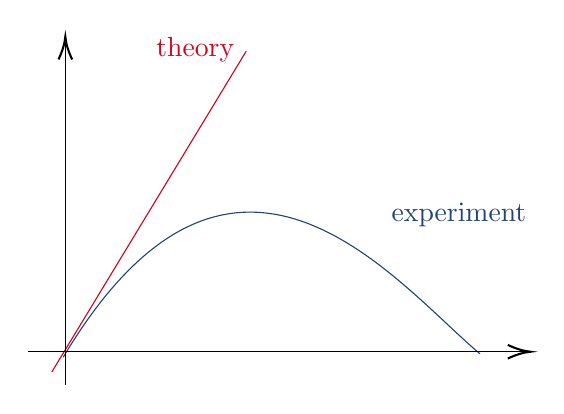
\begin{tikzpicture}[x=0.75pt,y=0.75pt,yscale=-1,xscale=1]
%uncomment if require: \path (0,300); %set diagram left start at 0, and has height of 300

%Straight Lines [id:da44773090746859867] 
\draw [color={rgb, 255:red, 208; green, 2; blue, 27 }  ,draw opacity=1 ]   (100.87,233.5) -- (194.5,79) ;
%Curve Lines [id:da7265875796819894] 
\draw [color={rgb, 255:red, 34; green, 68; blue, 114 }  ,draw opacity=1 ]   (106.37,226.38) .. controls (188.5,89) and (266.53,190.65) .. (307.14,224.76) ;
%Straight Lines [id:da8045363903004159] 
\draw    (89.5,223.76) -- (329.5,223.76) ;
\draw [shift={(331.5,223.76)}, rotate = 180] [color={rgb, 255:red, 0; green, 0; blue, 0 }  ][line width=0.75]    (10.93,-3.29) .. controls (6.95,-1.4) and (3.31,-0.3) .. (0,0) .. controls (3.31,0.3) and (6.95,1.4) .. (10.93,3.29)   ;
%Straight Lines [id:da5761614694400692] 
\draw    (107.37,240) -- (107.37,74) ;
\draw [shift={(107.37,72)}, rotate = 450] [color={rgb, 255:red, 0; green, 0; blue, 0 }  ][line width=0.75]    (10.93,-3.29) .. controls (6.95,-1.4) and (3.31,-0.3) .. (0,0) .. controls (3.31,0.3) and (6.95,1.4) .. (10.93,3.29)   ;

% Text Node
\draw (170,78) node  [color={rgb, 255:red, 208; green, 2; blue, 27 }  ,opacity=1 ] [align=left] {theory};
% Text Node
\draw (297,158) node  [color={rgb, 255:red, 34; green, 68; blue, 114 }  ,opacity=1 ] [align=left] {experiment};


\end{tikzpicture}
\end{figure}

This implies that the theory does not work for high energies. In order to have an unitary theory a requirement is 
\[\bar\sigma\leq\frac{4\pi}{s}\]
i.e. V-A theory preserves unitariety only if $\sqrt s\leq\sqrt{2\pi/G_F}\simeq 700$GeV. This implies that initial energies of particles in c.o.m. have to be smaller than $\approx 300$GeV.


\begin{figure}[H]
\centering


\tikzset{every picture/.style={line width=0.75pt}} %set default line width to 0.75pt        

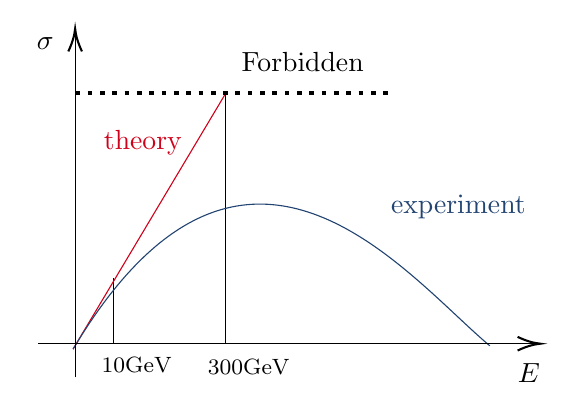
\begin{tikzpicture}[x=0.75pt,y=0.75pt,yscale=-1,xscale=1]
%uncomment if require: \path (0,300); %set diagram left start at 0, and has height of 300

%Straight Lines [id:da7811652857836433] 
\draw    (180,103) -- (180,224) ;
%Straight Lines [id:da7584225598218981] 
\draw    (126,192) -- (126,224) ;
%Straight Lines [id:da44773090746859867] 
\draw [color={rgb, 255:red, 208; green, 2; blue, 27 }  ,draw opacity=1 ]   (106.37,226.38) -- (180,103) ;
%Curve Lines [id:da7265875796819894] 
\draw [color={rgb, 255:red, 34; green, 68; blue, 114 }  ,draw opacity=1 ]   (106.37,226.38) .. controls (188.5,89) and (266.53,190.65) .. (307.14,224.76) ;
%Straight Lines [id:da8045363903004159] 
\draw    (89.5,223.76) -- (329.5,223.76) ;
\draw [shift={(331.5,223.76)}, rotate = 180] [color={rgb, 255:red, 0; green, 0; blue, 0 }  ][line width=0.75]    (10.93,-3.29) .. controls (6.95,-1.4) and (3.31,-0.3) .. (0,0) .. controls (3.31,0.3) and (6.95,1.4) .. (10.93,3.29)   ;
%Straight Lines [id:da5761614694400692] 
\draw    (107.37,240) -- (107.37,74) ;
\draw [shift={(107.37,72)}, rotate = 450] [color={rgb, 255:red, 0; green, 0; blue, 0 }  ][line width=0.75]    (10.93,-3.29) .. controls (6.95,-1.4) and (3.31,-0.3) .. (0,0) .. controls (3.31,0.3) and (6.95,1.4) .. (10.93,3.29)   ;
%Straight Lines [id:da1588459136106537] 
\draw [line width=1.5]  [dash pattern={on 1.69pt off 2.76pt}]  (107.5,103) -- (259.75,103) ;

% Text Node
\draw (140,127) node  [color={rgb, 255:red, 208; green, 2; blue, 27 }  ,opacity=1 ] [align=left] {theory};
% Text Node
\draw (292,158) node  [color={rgb, 255:red, 34; green, 68; blue, 114 }  ,opacity=1 ] [align=left] {experiment};
% Text Node
\draw (217,88) node   [align=left] {Forbidden};
% Text Node
\draw (326,238) node    {$E$};
% Text Node
\draw (93,79) node    {$\sigma $};
% Text Node
\draw (137,234) node  [font=\footnotesize] [align=left] {10GeV};
% Text Node
\draw (191,235) node  [font=\footnotesize] [align=left] {300GeV};


\end{tikzpicture}
\end{figure}

\subsubsection{Non renormalizabililty}

We saw that Fermi theory is not renormalizable, since $[G_F]=-2$ implies ultaviolet divergence at higher orders.
























\end{document}